\documentclass[12pt]{beamer}




\usetheme{CambridgeUS}
\usecolortheme{seahorse}

\usepackage[utf8]{inputenc}
\usepackage[french]{babel}
\usepackage{graphicx}
\usepackage{amsmath}

\title{E-Learning : Apprentissage ou Distraction?}
\author{25019-25048-25057-25188}
\institute{Institut Supérieur du Numérique (SupNum)}
\date{\today}
\centering
\begin{document}


\frame{\titlepage}


\begin{frame}
\centering
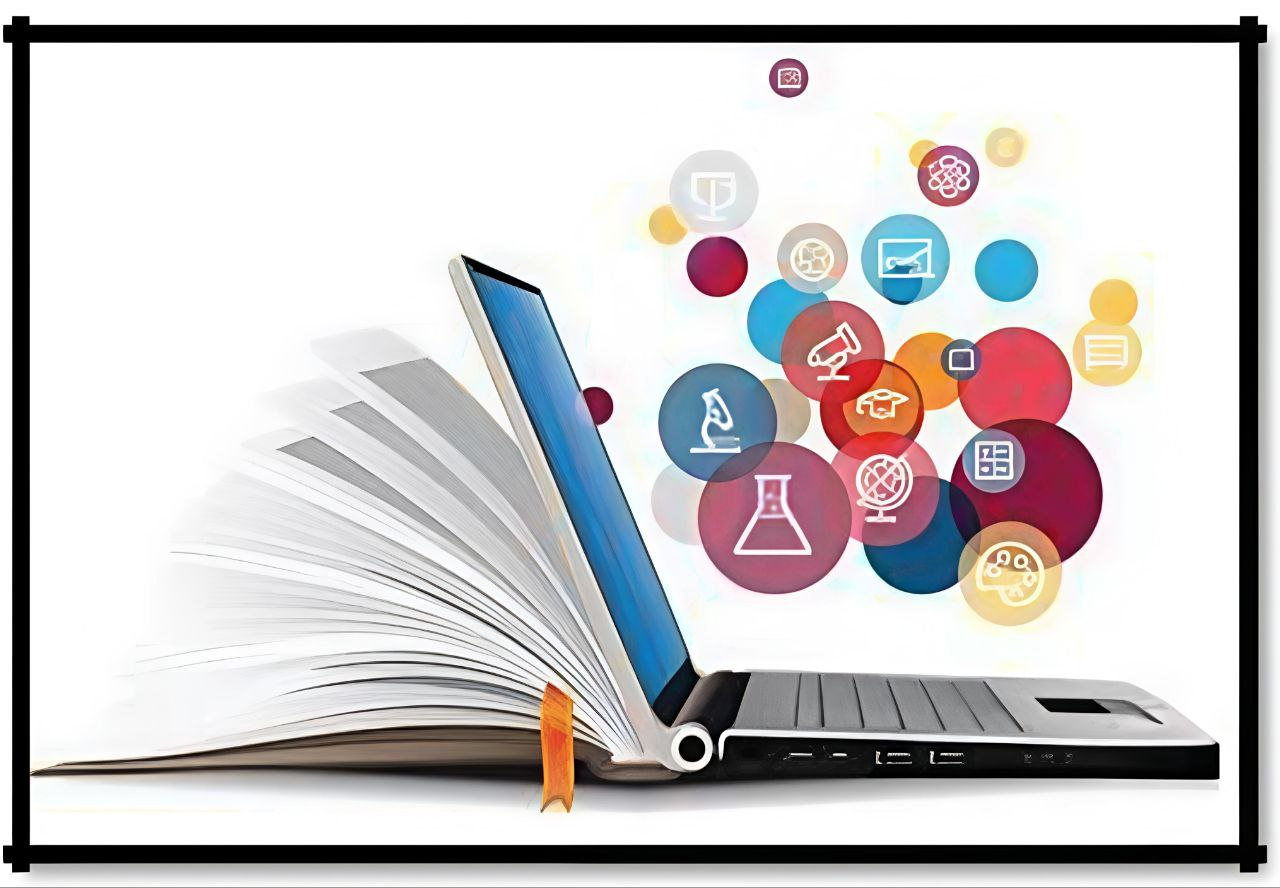
\includegraphics[width=0.7\textwidth]{1.jpg}
\end{frame}


\begin{frame}{Résumé}
Ce rapport étudie comment les nouveaux outils numériques influencent le comportement des étudiants.
Nous analysons l’évolution depuis la crise sanitaire et observons l’impact du e-learning sur la concentration et l’efficacité académique.
L’objectif est de comprendre dans quelle mesure le numérique constitue un soutien à l’apprentissage ou une source potentielle de distraction.
\end{frame}


\begin{frame}{Introduction}
La transformation numérique a changé le monde de l'éducation de façon permanente.

Selon le rapport officiel de l'UNESCO (2020), plus de 1,6 milliard d'étudiants ont été obligés de passer au numérique à cause du COVID-19.

Aujourd'hui, le numérique reste l'outil principal dans les instituts universitaires.
\end{frame}


\begin{frame}{Problématique}
Le problème principal est de savoir comment l'utilisation constante d'Internet influence la concentration des apprenants.

Est-ce que la possession massive de smartphones est une aide ou une source de distraction majeure pendant les études ?


\end{frame}





\begin{frame}{Hypothèses de recherche}
Considérant que & 95\% & des étudiants possèdent un smartphone, nous supposons que l'impact du numérique varie selon l'âge. Cette hypothèse nous amène à analyser la répartition de l'usage des plateformes pour identifier la catégorie la plus exposée au risque de distraction.
\end{frame}

\begin{frame}{Analyse par tranche d’âge}
Le tableau ci-dessous présente une synthèse comparative basée sur une analyse descriptive des usages numériques:


\centering
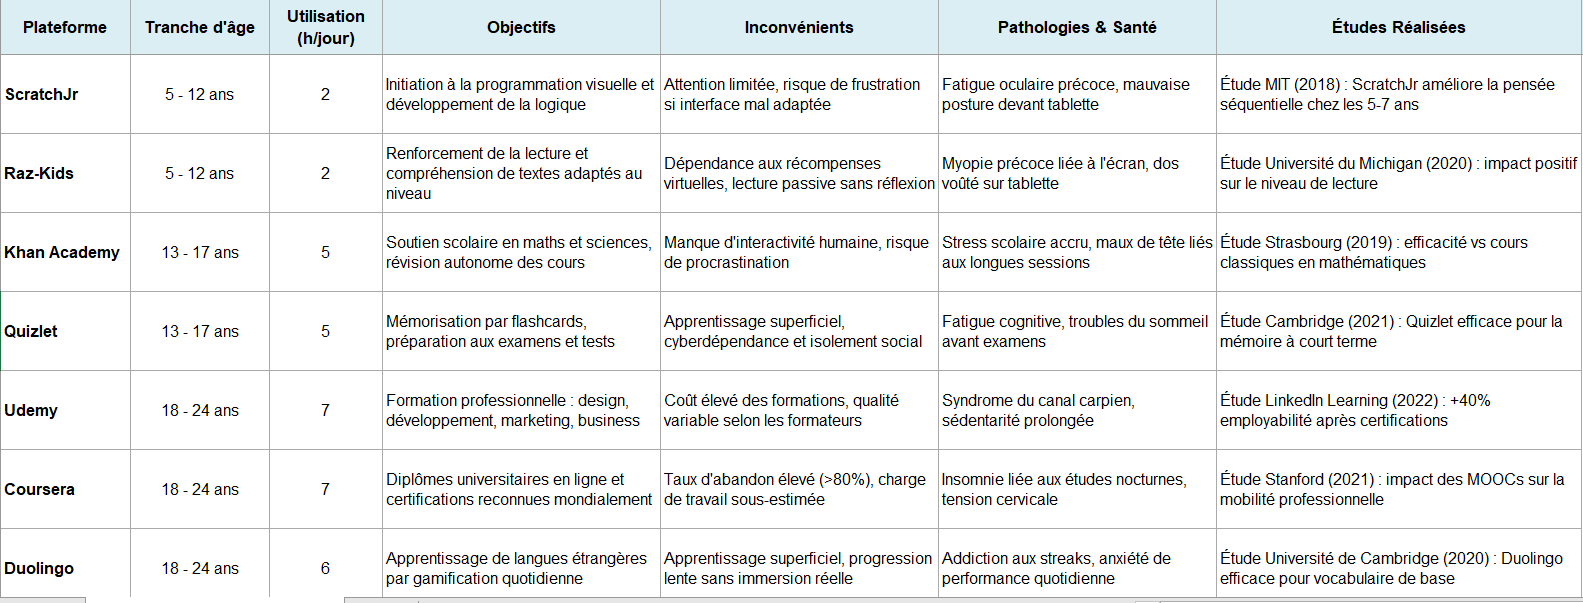
\includegraphics[width=0.9\paperwidth]{5.png}
\end{frame}
\begin{frame}{Analyse par tranche d’âge(2)}
\centering
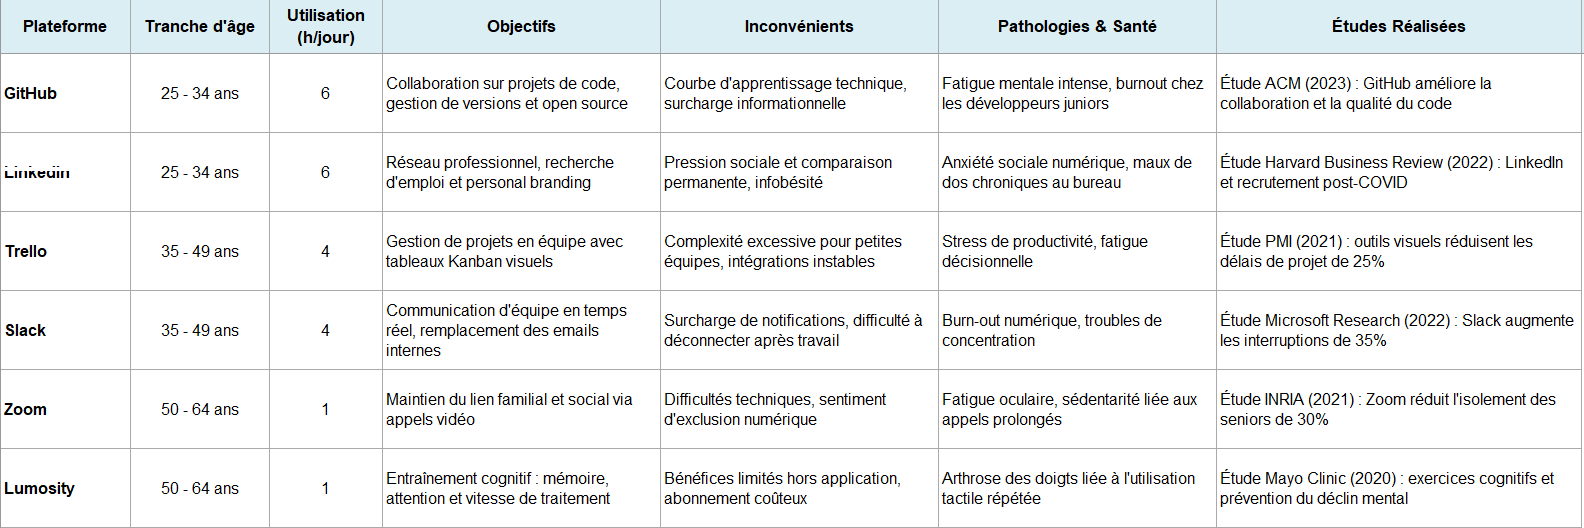
\includegraphics[width=0.9\paperwidth]{6.png}

\end{frame}

\begin{frame}{Statistiques principales}


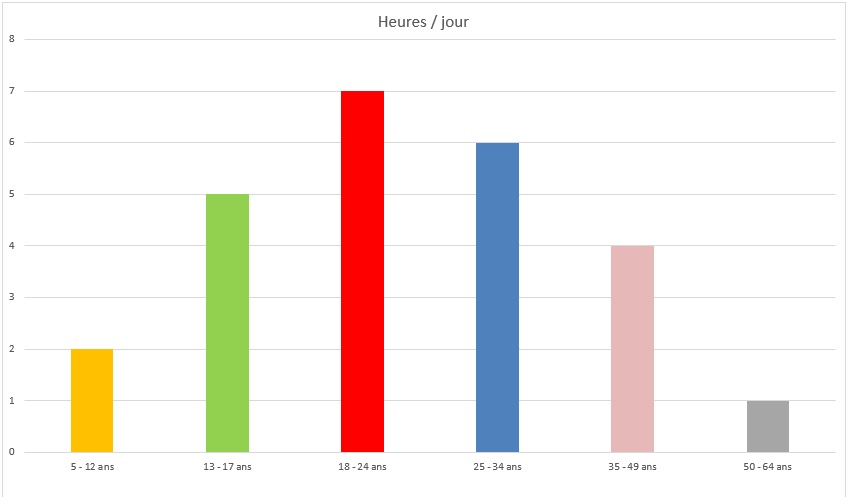
\includegraphics[width=\linewidth]{4.png}
\end{frame}

\begin{frame}{Conclusion}
Les plateformes numériques apportent des bénéfices importants en matière d’apprentissage, de compétences et de communication.
Cependant, un usage excessif peut engendrer une fatigue cognitive, visuelle et du stress numérique.
Un usage équilibré demeure donc essentiel.

La technologie est un outil puissant.

Cependant, elle nécessite une gestion stricte pour éviter la perte de concentration profonde.
\end{frame}


\begin{frame}{Références}
\begin{thebibliography}{9}
\bibitem{} UNESCO (2020). Rapport mondial sur l'éducation.
\bibitem{} Pew Research Center (2023). Digital habits among teens.
\end{thebibliography}
\end{frame}

\end{document}
Les plateformes numériques apportent des bénéfices importants en matière d’apprentissage, de compétences et de communication.
Cependant, un usage excessif peut engendrer une fatigue cognitive, visuelle et du stress numérique.
Un usage équilibré demeure donc essentiel.

La technologie est un outil puissant.

Cependant, elle nécessite une gestion stricte pour éviter la perte de concentration profonde.
\end{frame}


\begin{frame}{Références}
\begin{thebibliography}{9}
\bibitem{} UNESCO (2020). Rapport mondial sur l'éducation.
\bibitem{} Pew Research Center (2023). Digital habits among teens.
\end{thebibliography}
\end{frame}

\end{document}
